\documentclass{article}

\usepackage{tikz}
\usepackage{tikz}
\usepackage{pgfplots}
\usetikzlibrary{backgrounds, positioning, fit}
\usetikzlibrary{shapes.geometric}
\usetikzlibrary{patterns}

%% put tikzlibrary below if necessary

% set up externalization
\usetikzlibrary{external}
\tikzset{external/system call={latex \tikzexternalcheckshellescape -halt-on-error
-interaction=batchmode -jobname "\image" "\texsource";
dvips -o "\image".ps "\image".dvi;
ps2eps "\image.ps"}}
\tikzexternalize



\begin{document}

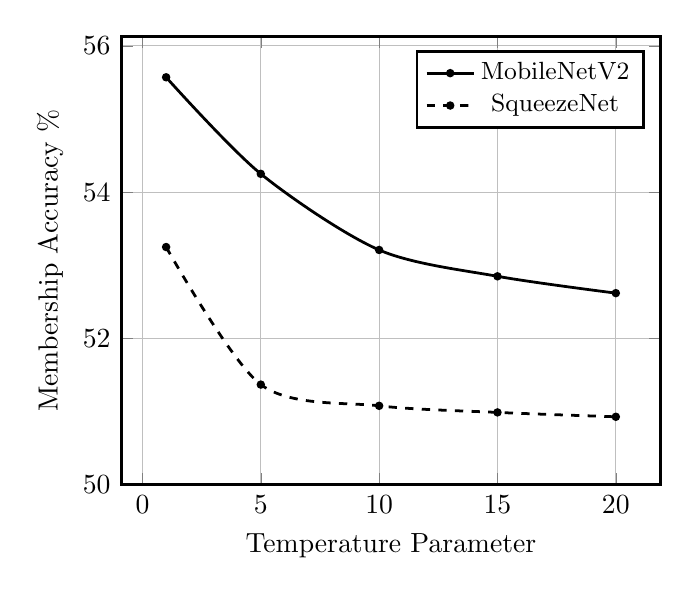
\begin{tikzpicture}
\begin{axis}[
legend style={font=\small},
legend pos =  north east,
line width=1.0pt,
mark size=1.0pt,
ymin=50,
legend entries={MobileNetV2, SqueezeNet},
ylabel={Membership Accuracy \%},
xlabel={Temperature Parameter},
xlabel style={font=\large},
ylabel style={font=\large},
xlabel near ticks,
ylabel near ticks,
% extra x ticks={1,10,...,400},
% extra y ticks={0,0.5,...,10},
% extra y tick labels={},
% extra x tick labels={},
% extra x tick style={grid=major},
% extra y tick style={grid=major},
grid=major
]
\addplot[
    color=black,
    solid,
    mark=*,
    mark options={solid},
    smooth
    ]
    coordinates {
    (1,55.57)(5,54.25)(10,53.21)(15,52.85)(20,52.62)
      };
\addplot[
      color=black,
      dashed,
      mark=*,
      mark options={solid},
      smooth
    ]
    coordinates {
    (1,53.25)(5,51.37)(10,51.08)(15,50.99)(20,50.93)
      };
\end{axis}
\end{tikzpicture}


\end{document}
